\subsection{Cellular Automata}
    Cellular Automata are parallel computing models, whose evolution
    is defined by local rules. A cellular automaton can be thought as
    a $d$-dimensional space, called \emph{cellular space}, subdivided
    in regular cells of uniform shape and size. Each cell embeds a
    \emph{finite automaton}, one of the most simple and well known
    computational models, which can assume a finite number of
    states. At time $t=0$, cells are in arbitrary states and the CA
    evolves step by step by changing the states of the cells at
    discrete time steps, by applying the same local rule of evolution,
    i.e. the cell's \emph{transition function}, simultaneously
    (i.e. in parallel) to each cell of the CA. Input for the cell is
    given by the states of a predefined (usually small) set of
    neighboring cells, which is assumed invariant in space and time
    (cf. Figures \ref{fig:2Dneighborhood} and \ref{fig:3Dneighborhood}
    for examples of 2D and 3D neighborhoods, respectively).

    %% It is possible to identify an informal definition of cellular
    %% automaton by simply listing its main properties:

    %% \begin{itemize}
    %% \item It is formed by a $d$-dimensional space (i.e. the
    %%   \emph{cellular space}), partitioned into cells of uniform shape
    %%   and size (e.g. triangles, squares, hexagons, cubes, etc. - see
    %%   Figure \ref{fig:cellularspaces});
    %% \item The number of cell's states is finite;
    %% \item The evolution occurs through discrete steps;
    %% \item Each cell changes state simultaneously to each other
    %%   (i.e. they change state concurrently, in parallel) thanks to the
    %%   application of the cell's \emph{transition function};
    %% \item The cell's state transition depends on the states of a set
    %%   of neighboring cells;
    %% \item The evolving cell is called \emph{central cell} and can
    %%   belong to its neighborhood;
    %% \item The neighboring relationship is local, uniform and invariant
    %%   over time (see Figures \ref{fig:2Dneighborhood} and
    %%   \ref{fig:3Dneighborhood} for examples of 2D and 3D
    %%   neighborhoods, respectively).
    %% \end{itemize}

    \begin{figure}
      \begin{center}
        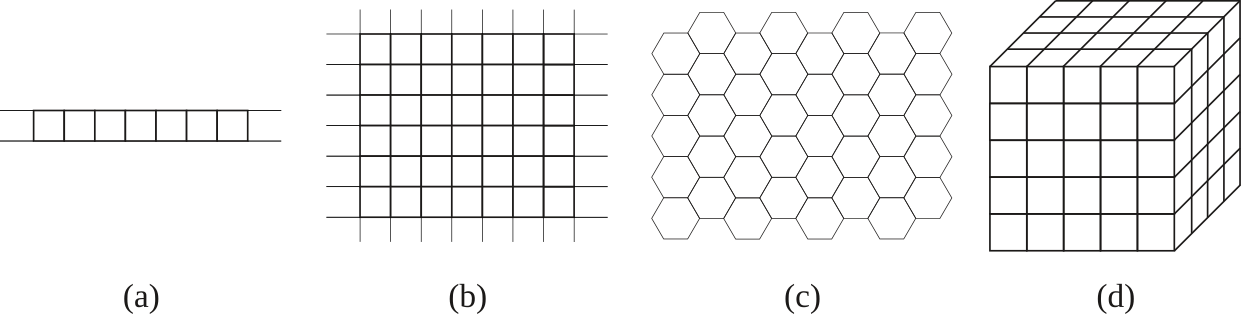
\includegraphics[scale=0.5]{./images/cellularspaces.png}
        \caption{Example of cellular spaces: (a) one-dimensional, (b)
          two-dimensional with square cells, (c) two-dimensional with
          hexagonal cells, (d) three-dimensional with cubic cells.}
        \label{fig:cellularspaces}
      \end{center}
    \end{figure}

    \begin{figure}
      \begin{center}
        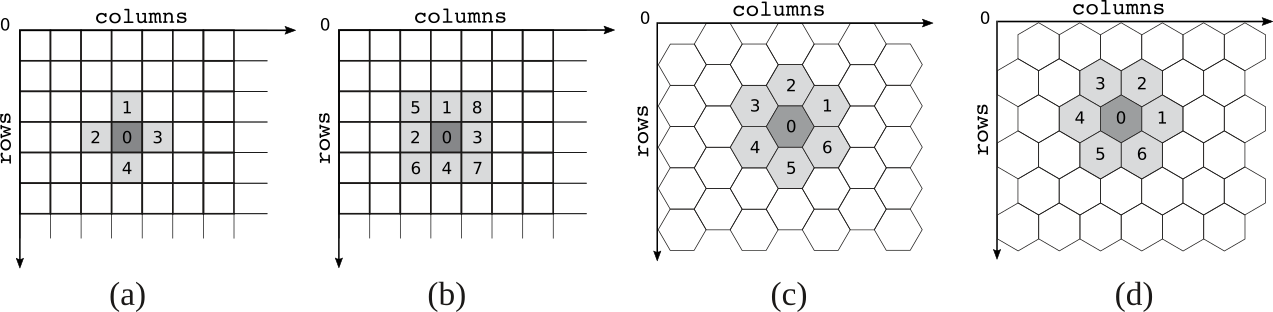
\includegraphics[scale=0.5]{./images/2Dneighborhoods.png}
        \caption{Examples of von Neumann (a) and Moore (b)
          neighborhoods for two-dimensional CA with square
          cells. Examples of (Moore) neighborhoods are also shows for
          hexagonal CA, both for the cases of horizontal (c) and
          vertical (d) cells orientation. Central cell is represented
          in dark gray, while adjacent cells are in light gray. A
          numerical identifier can optionally be assigned to a cell
          within a neighborhood. Note that the central cell can
          optionally belong to its own neighborhood.}
        \label{fig:2Dneighborhood}
      \end{center}
    \end{figure}

    \begin{figure}
      \begin{center}
        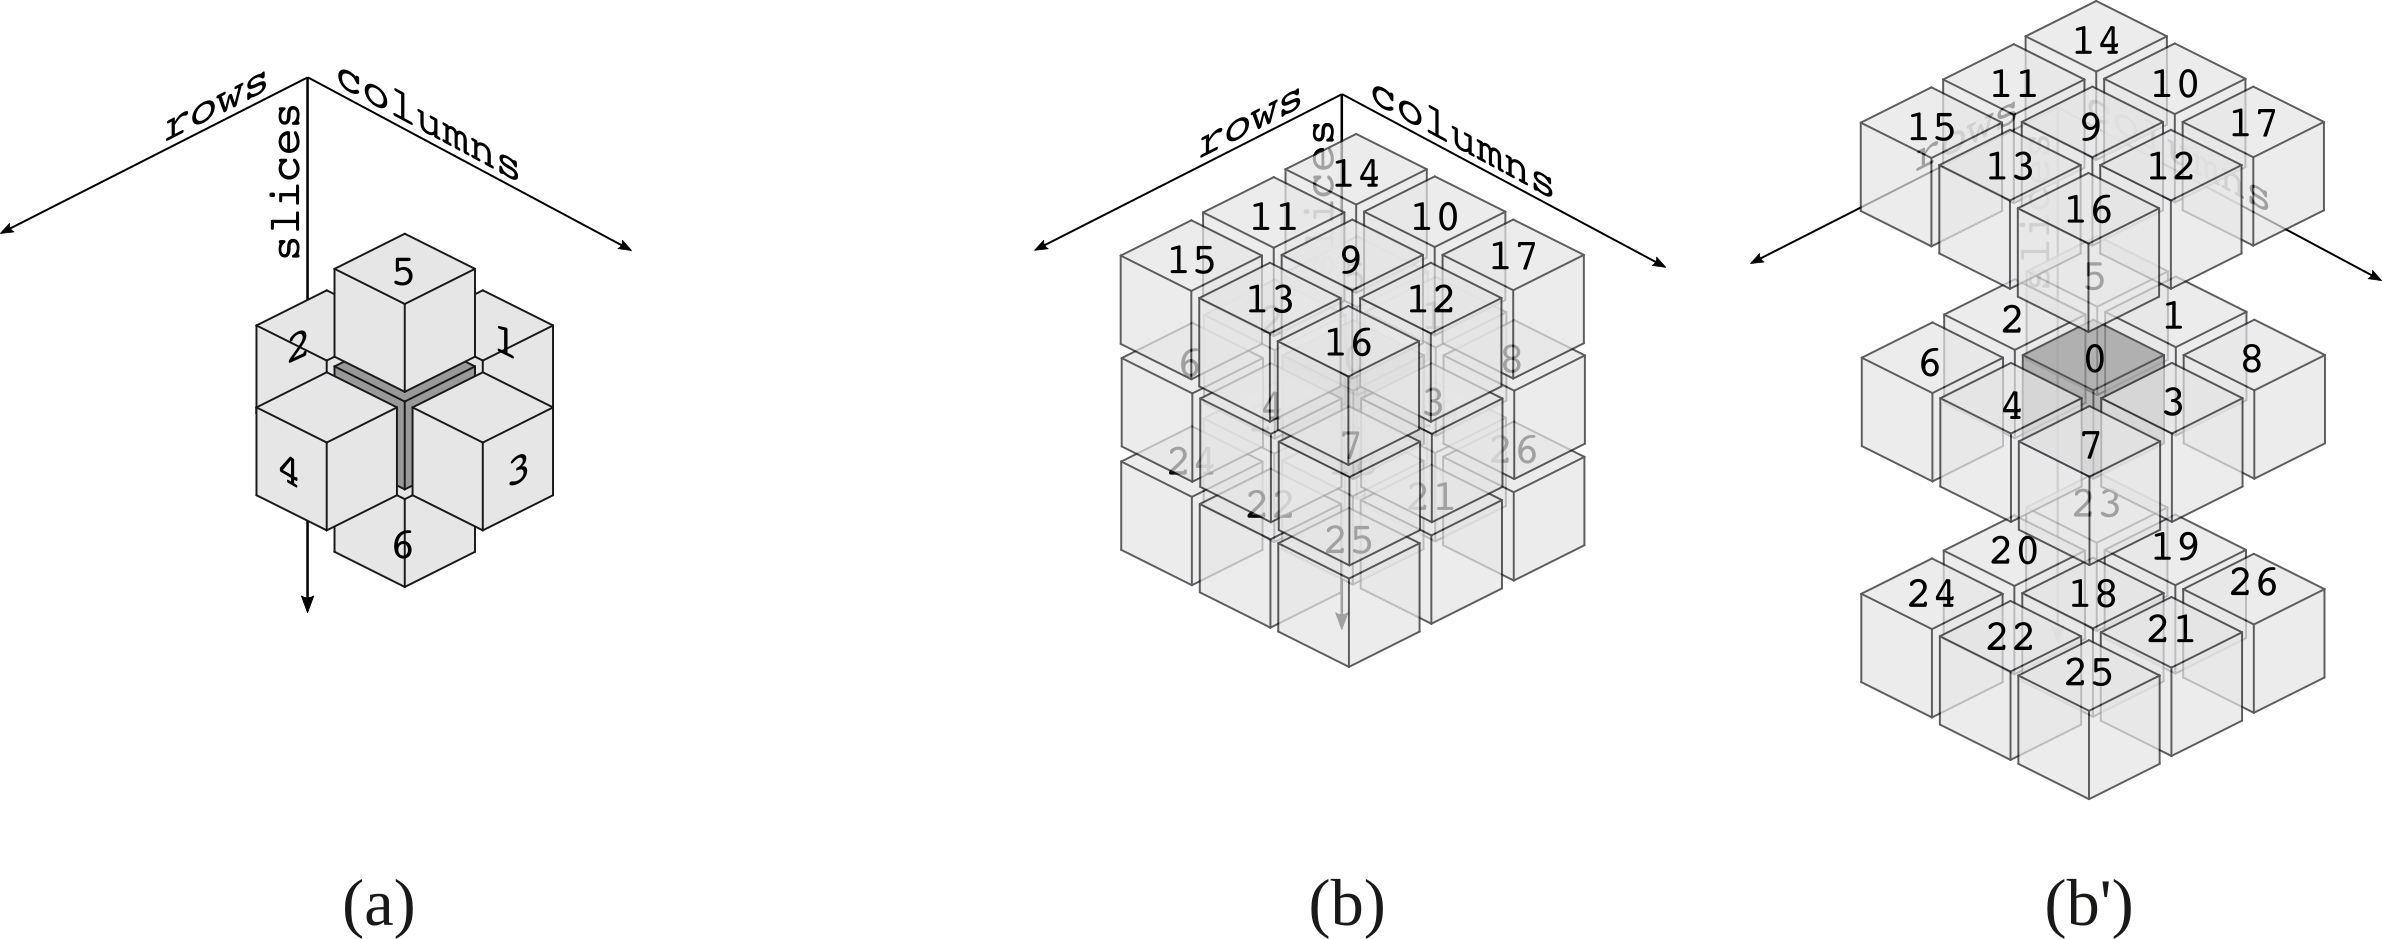
\includegraphics[width=0.45454545\textwidth]{./images/3Dneighborhoods.png}
        \caption{Examples of von Neumann (a) and Moore (b, b')
          neighborhoods for three-dimensional CA with cubic
          cells. Central cell is represented in dark gray, while
          adjacent cells are in light gray. As for the case of
          two-dimensional neighborhoods, a numerical identifier can
          optionally be assigned to a cell within a three-dimensional
          neighborhood.}
        \label{fig:3Dneighborhood}
      \end{center}
    \end{figure}

    Despite their simple definition, CA can exhibit very interesting
    complex global behaviors. Moreover, from a computational point of
    view, they are equivalent to Turing Machines. This means, in
    principle, that everything that can be computed can also be by
    means of a cellular automaton (Church Turing thesis). Thanks to
    their \emph{computational universality}, CA gained a great
    consideration among the Scientific Community and were employed for
    solving a great variety of different complex problems. Cellular
    Automata are formally defined as a quadruple:

    $$A = <R,X,Q,\sigma>$$

    \noindent where:

    \begin{itemize}
    \item $R = \{i = (i_0,i_1,...,i_{d-1}) \; | \; i_k \in \mathbb{Z} \;\; \forall k =
      0,1,...,d-1\}$ is the set of points, with integer coordinates, which
      defines the $d$-dimensional cellular space;

    \item $X = \{\xi_0,\xi_1\,...\xi_{m-1}\}$ is the finite set of $m$
      $d$-dimensional vectors
      \[ \xi_j = \{\xi_{j_0},\xi_{j_1},...\xi_{j_{d-1}}\} \]
      that define the set
      \[ N(X,i) = \{i + \xi_0,i + \xi_1,...,i + \xi_{m-1}\} \]
      of coordinates of cells belonging the the central cell's
      neighborhood. In other words, $X$ represents the geometrical
      pattern that specifies the neighborhood relationship;

    \item $Q$ is the finite set of states of the cell;

    \item $\sigma : Q^m \rightarrow Q$ is the cell's transition
      function. Note that, a cell $i$ is said to be in a
      \emph{quiescent state}, $q_0 \in Q$, if all its neighbouring
      cell are in the same state and $\sigma(q_0, q_0, \ldots, q_0) = q_0$.

    \end{itemize}
    
    Let $C = \{ c | c: R \rightarrow Q \}$ be the set of global
    configurations of the CA, and $c(i)$ the state of the cell $i$ in
    the configuration $c$. The CA \emph{global trnasition function},
    which applies the cell transition function to all the cells in
    $R$, is defined as:
    $$
    \begin{array}{r}
      \tau : C \longrightarrow C \\
      c \mapsto \tau(c) \\
    \end{array}
    $$
    where
    $$
    \tau(c(i)) = \sigma(c(N(X, i))) = \sigma(c(i + \xi_0), c(i + \xi_1), \ldots, c(i + \xi_{m-1}))
    $$

    \noindent and the global evolution of the CA is obtained by
    applying the global transition function $\tau$ step by step.


  \subsection{Extended Cellular Automata}
    Extended Cellular Automata \cite{DiGregorio&Serra-1999} represents
    an extension of the original CA computational paradighm. XCA were
    firstly applied to the simulation of basaltic lava flows in the
    80's \cite{Crisci&al-1982} and many subsequent examples of
    application shown that the approach behind XCA can greatly make
    more straightforward the modeling of some complex systems.

    Informally, XCA, compared to classical CA, are different because
    of the following reasons:

    \begin{itemize}

    \item The cell's state is decomposed in \emph{substates}, each of them
      representing the set of admissible values of a given characteristic
      assumed to be relevant for the modeled system and its evolution
      (e.g., lava temperature, lava thickness, etc, in the case of a lava
      flow model). The set of states for the cell is simply obtained as
      the Cartesian product of the considered substates.

    \item As the cell's state can be decomposed in substates, also the
      transition function can be split into \emph{elementary processes},
      each of them representing a particular aspect that rules the dynamic
      of the considered phenomenon. In turn, \emph{elementary processes}
      can be split into \emph{local interactions}, which refer to rules
      that deal with interactions among substates of the cell with
      neighbor ones (e.g., mass exchange with neighbors) and
      \emph{internal transformations}, defined as the changes in the
      values of the substates due only to interactions among substates
      inside the cell (e.g. the solidification of the lava inside the cell
      due to the temperature drop).

    \item A set of \emph{parameters}, commonly used to characterize the
      dynamic behaviors of the considered phenomenon, can be defined.

    \item Global operations can also be allowed (e.g. to model external
      influences that can not easily be described in terms of local
      interactions, or to perform reductions over the whole, or a subset
      of, the cellular space). They are often referred as \emph{steering}
      operations.

    \end{itemize}

    Formally, a XCA is defined as a 7-tuple:

    $$ A = <R,X,Q,P,\sigma,\Gamma,\gamma>$$

    \noindent where:

    \begin{itemize}

    \item $R$ is the $d$-dimensional cellular space.

    \item $\Gamma \subseteq R$ is the region over which steering is applied.

    \item $X$ is the geometrical pattern that specifies the neighborhood
      relationship; $m = |X|$ represent the number of elements in the set
      $X$, i.e. the number of neighbors for the central cell.

    \item $Q = Q_0 \times Q_1 \times....\times Q_{n-1}$ is the set of
      cell's states, expressed as Cartesian product of the $n$ considered
      \emph{substates} $Q_0 \times Q_1 \times....\times Q_{n-1}$.

    \item $P = {p_0,p_1,....,p_{p-1}}$ is the set of CA
      \emph{parameters}.They can allow a fine tuning of the XCA model,
      with the purpose of reproducing different dynamical behaviors of
      the phenomenon of interest.

    \item $\psi : Q^{|R|} \rightarrow Q^{|R|}$ is the global function
      which define the initial conditions of the system.
      
    \item $\sigma : Q^m \rightarrow Q$ is the cell's transition function.
      It is split in $s$ \emph{elementary processes}, $\sigma_0,\sigma_1,
      ..., \sigma_{s-1}$, each one describing a particular aspect ruling
      the dynamic of the considered system.

    \item $\gamma: Q^{|\Gamma|} \rightarrow Q^{|\Gamma|} \times
      \mathbb{R}$ is the (global) steering function.

    \end{itemize}

    The initial conditions of the system are obtained by preliminarly
    applying the $\psi$ initialization function. Then, if $\tau$
    represents the function which applyes the transition function
    $\sigma$ to all the cells in $R$, as for the CA case, and $\gamma$
    the XCA steering function, the XCA evolution is obatained by
    applying the $\Phi = \tau \circ \gamma$ XCA global transition
    function at discrete time steps.
